\documentclass[10.5pt]{article}
\usepackage{amsmath, amsfonts, amssymb,amsthm}
\usepackage[includeheadfoot]{geometry} % For page dimensions
\usepackage{fancyhdr}
\usepackage{enumerate} % For custom lists
\usepackage{tikz-cd}
\usepackage{graphicx}

\fancyhf{}
\lhead{MAT1301 hw8}
\rhead{Tighe McAsey - 1008309420}
\pagestyle{fancy}

% Page dimensions
\geometry{a4paper, margin=1in}

\theoremstyle{definition}
\newtheorem{pb}{}
\usepackage{tikz-cd, stackengine}

% Commands:
\tikzset{
  curarrow/.style={
  rounded corners=8pt,
  execute at begin to={every node/.style={fill=red}},
    to path={-- ([xshift=-50pt]\tikztostart.center)
    |- (#1) node[fill=white] {$\scriptstyle \delta$}
    -| ([xshift=50pt]\tikztotarget.center)
    -- (\tikztotarget)}
    }
}

\newcommand{\set}[1]{\{#1\}}
\newcommand{\gen}[1]{\langle#1\rangle}
\newcommand{\abs}[1]{\left\vert#1\right\vert}
\newcommand{\norm}[1]{\lvert\lvert#1\rvert\rvert}
\newcommand{\tand}{\text{ and }}
\newcommand{\tor}{\text{ or }}
\newcommand{\pd}{\frac{\partial}{\partial x_j}}
\newcommand{\px}{\frac{\partial}{\partial x}}
\newcommand{\py}{\frac{\partial}{\partial y}}
\newcommand{\pz}{\frac{\partial}{\partial z}}
\newcommand{\ppx}{\frac{\partial^2}{\partial x^2}}
\newcommand{\ppy}{\frac{\partial^2}{\partial y^2}}
\newcommand{\ppz}{\frac{\partial^2}{\partial z^2}}
\newcommand{\hess}{\operatorname{Hess}}

\begin{document}
    \begin{pb}
        Write \(S^{n} = \set{(x_0,\hdots,x_n) \mid \sum x_j^2 = 1}\), then we may define the surjective map \(S^n \to D^n\) as \(q: (x_0,\hdots,x_n) \mapsto (x_1,\hdots,x_n)\), then take \(\pi: D^n \to D^n/\partial D^n \cong S^n\). This map is also surjective, it follows that \(\pi\circ q: S^n \to S^n\) is surjective, and it must have degree zero, since it factors through \(D^n\), and \(H_n(D^n) = 0\). \qed
    \end{pb}
    \begin{pb}
        \textbf{(a)} Suppose \(g: S^n \to S^n\) does not have a fixed point, then \(g\) is homotopic to the antipodal map \(r\) via
        \begin{align*}
            H(x,t) = \frac{(1-t)g(x) - tx}{\abs{(1-t)g(x) - tx}}
        \end{align*}
        But \(g\) being non surjective has some \(y \in S^n \setminus \operatorname{Im}g\), thus factors through
        \begin{align*}
            S^n \overset{g}{\longrightarrow} S^n\setminus \set{y} \hookrightarrow S^n
        \end{align*}
        where we identify \(g\) with \(\iota \circ g\). Applying the homology functor, we have \(S^n \setminus \set{y} \cong \mathbb{R}^n\), so that \(g\) factors through zero, and thus \(\deg r = \deg g = 0\), but \(\deg r = \pm 1\). \qed

        \textbf{(b)} Write \(S^n = D^n_U \cup_{\partial D^n} D^n_L\) as the union of the upper and lower hemispheres, then define
        \begin{align*}
            g:S^n &\to S^n \\
            g\vert_{D^n_U}: D^n_U \overset{f}{\to} D^n_L \quad & \quad  g\vert_{D^n_L}: D^n_L \overset{f}{\to} D^n_L
        \end{align*}
        Then \(g\) is not surjective, hence by part (a) has a fixed point, moreover the fixed point must be in the bottom hemisphere by definition of \(g\). This implies that \(g\vert_{D_L} = f\) has a fixed point. \qed
    \end{pb}
    \begin{pb}
        \textbf{(a)} We can give \(X\) a CW structure by letting \(X^1 = S^1\) which is \(D^1 = I\) gluing either boundary to the same point, and \(X^2 = D^2 \cup_{\phi} S^1\), where \(\phi: \partial D^2 = S^1 \to X^1 = S^1\) is the map \(z \mapsto z^3\), which notably has degree \(3\). This lets us compute the Homology using the CW structure, namely we have computed the chain complex is
        \begin{equation*}
            \begin{tikzcd}
                \gen{e_2} \arrow[r,"e_2 \mapsto 3e_1"] & \gen{e_1} \arrow[r,"e_1 \mapsto e_0 - e_0"] &\gen{e_0}
            \end{tikzcd}
        \end{equation*}
        So, the homology is given by \(H_2(X;\mathbb{Z}) = 0, H_1(X; \mathbb{Z}) \cong \mathbb{Z}/3 \mathbb{Z}\) and \(H_0(X;\mathbb{Z}) \cong \mathbb{Z}\) \qed

        \textbf{(b)} We can use the above approach, but we tensor the cellular chain complex for \(X\) by \(\mathbb{Z}/3 \mathbb{Z}\), this makes the above chain complex into
        \begin{equation*}
            \begin{tikzcd}
                \gen{e_2} \otimes \mathbb{Z}/3 \mathbb{Z} \arrow[r,"0"] & \gen{e_1} \otimes \mathbb{Z}/3 \mathbb{Z} \arrow[r,"0"] &\gen{e_0}\otimes \mathbb{Z}/3 \mathbb{Z}
            \end{tikzcd}
        \end{equation*}
        since \(e_2 \otimes 1 \mapsto 3 e_2 \otimes 1 = e_2 \otimes 3 = 0\) in the first differential, then each term can be identified with \(\mathbb{Z}/3 \mathbb{Z}\), since each of the maps are zero, we get \(H_n(X;\mathbb{Z}/3 \mathbb{Z}) = C_n^{\text{CW}} \otimes \mathbb{Z}/3 \mathbb{Z} \cong \mathbb{Z}/3 \mathbb{Z}\), so that \(H_j(X; \mathbb{Z}/ 3 \mathbb{Z}) = \mathbb{Z}/3 \mathbb{Z}\) if \(j \leq 2\) or \(0\) if \(j > 2\). \qed
    \end{pb}
    \newpage

    \begin{pb}
        The idea is to realize the trefoil as a torus knot, then cutting it out of the solid torus with filled meridian, and enclosing the removed section can still be given a CW complex \(X\) similar to that of the solid torus with filled meridian. We can then deformation retract the interior of the tube enclosing the knot complement to the tube itself, and project the rest of \(\mathbb{R}^3\) in the \(z\) direction onto \(\mathbb{R}^2 \cup X\) where \(X\) is this modified solid torus CW complex, then we can simply project \(\mathbb{R}^2\) radially onto \(X\). To understand this construction I will first do it for \(S^1\) embedded in the torus, then construct the more complicated CW complex for the trefoil in the same way. The homotopy has already been described, here is the CW complex.

        \begin{figure}[h]
            \begin{center}
                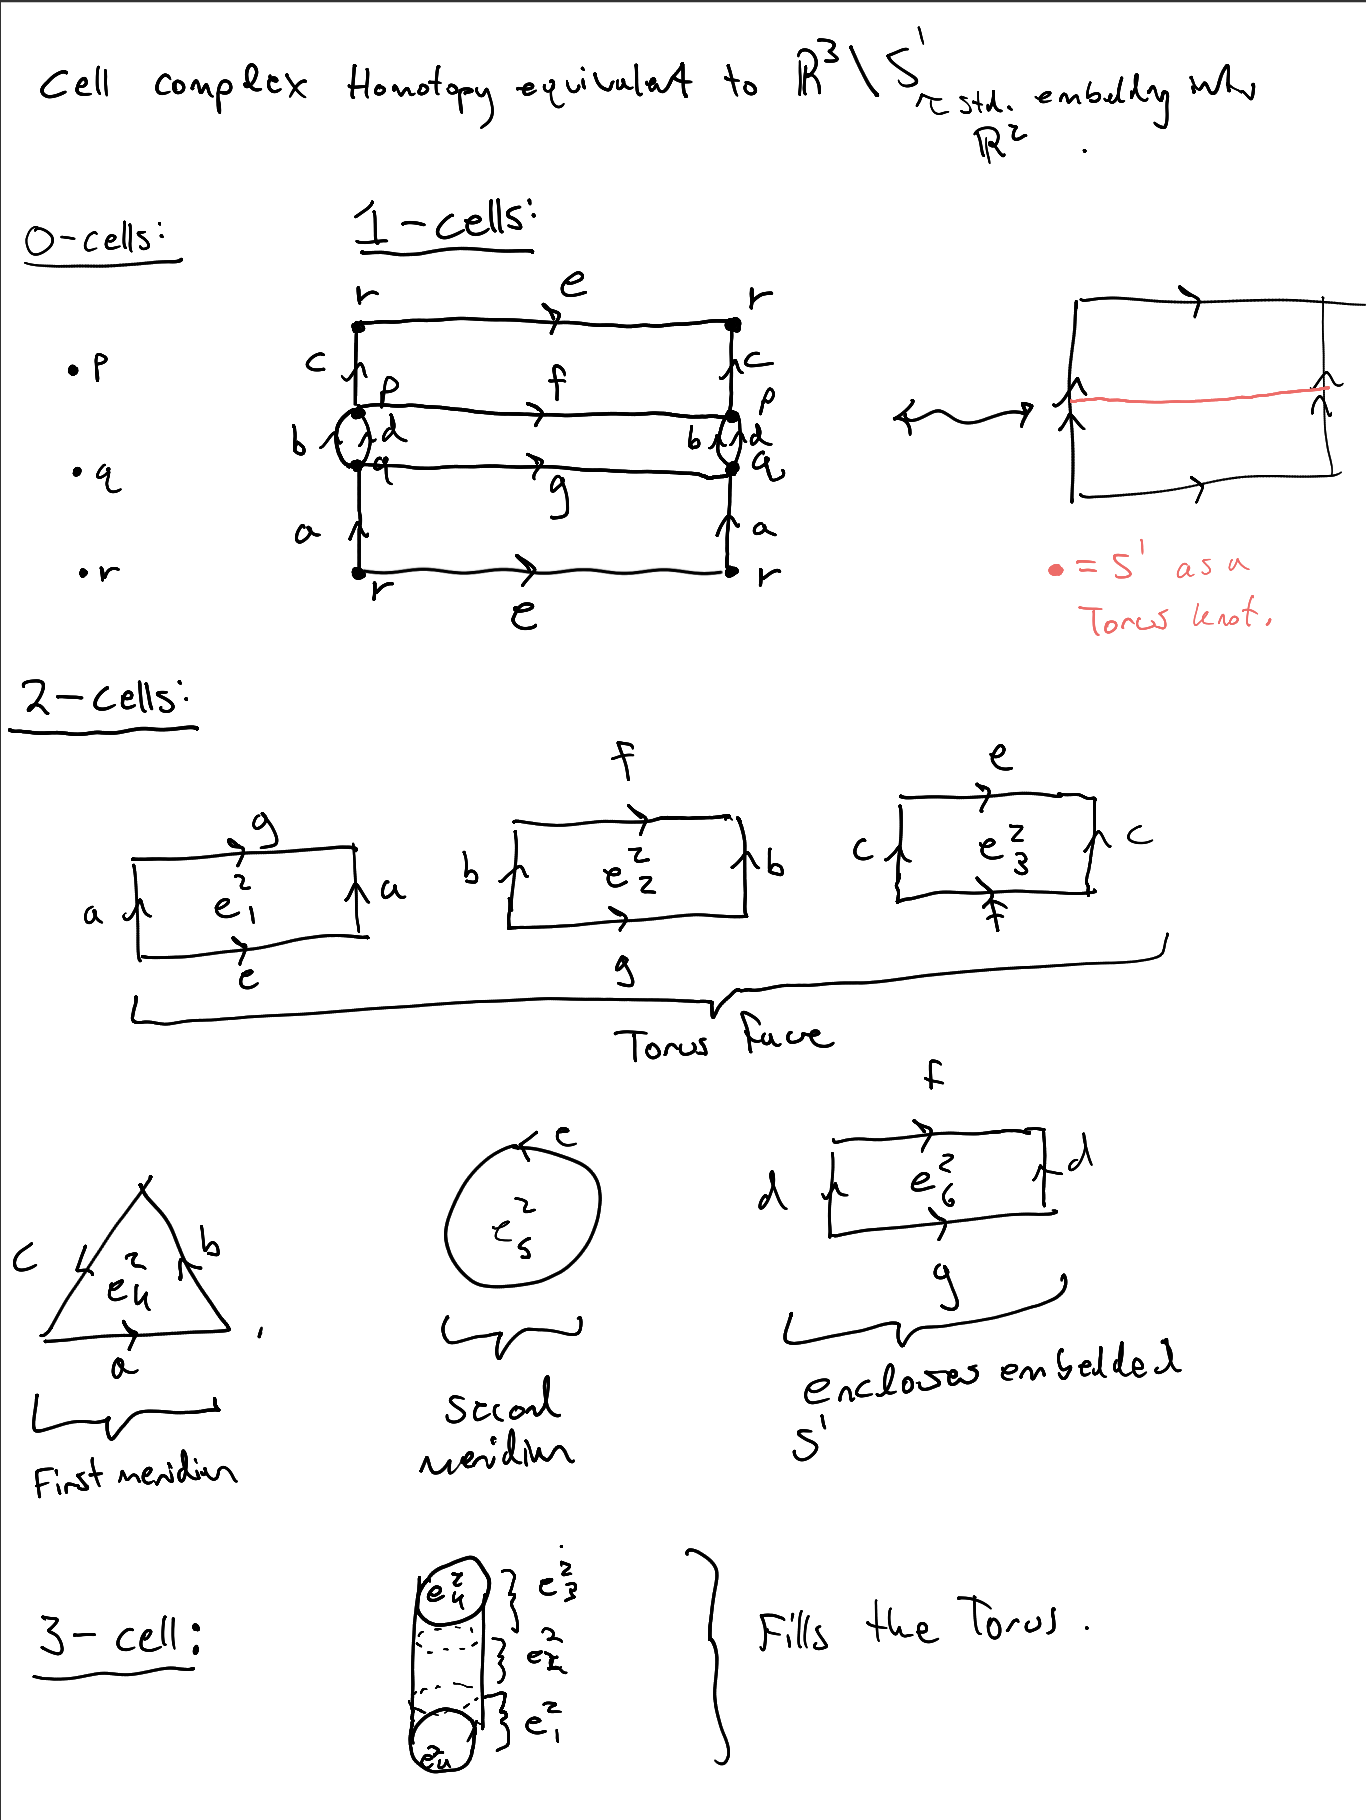
\includegraphics[width=0.9\linewidth]{figures/Figure1.png}
            \end{center}
        \end{figure}
        \begin{figure}[h]
            \begin{center}
                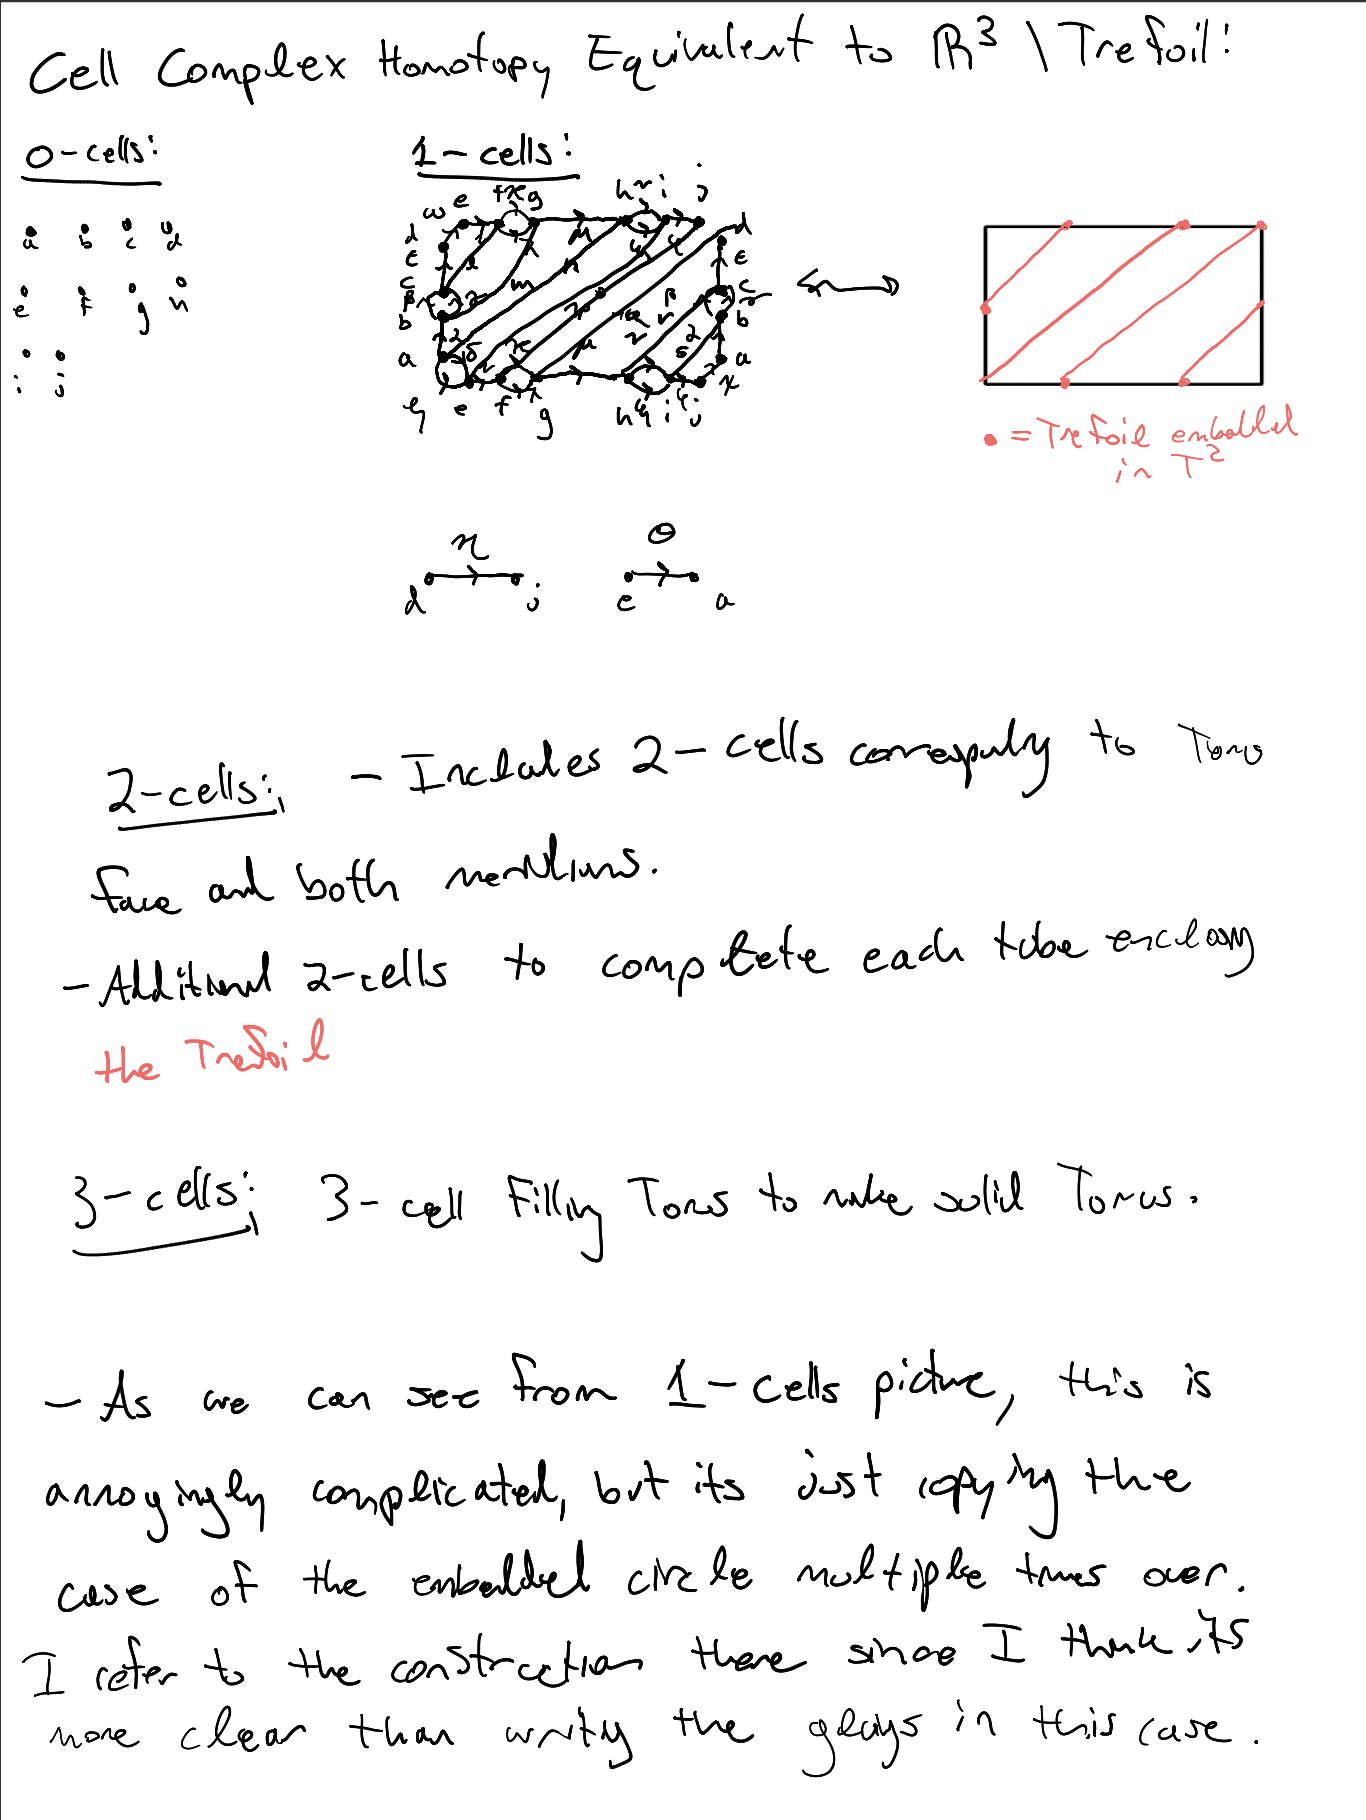
\includegraphics[width=0.9\linewidth]{figures/Figure2.png}
            \end{center}
        \end{figure}
    \end{pb}
    \newpage

    \begin{pb}
        \textbf{(a)} Begin by fixing an isomorphism \(H_2(T^2) \cong \mathbb{Z}\) and an isomorphism \(H_2(S^2) \cong \mathbb{Z}\), we define the degree of \(f: T^2 \to S^2\) to be the image of \(f_*(1)\) using these identifications with \(\mathbb{Z}\). We define the local degree using \(V \supset \set{y}\), and \(U\) such that \(x \in U \subset (f^{-1}(y) \setminus \set{x})^c\), then \(\deg_x f\) is defined to be the image of \(f_*(1): \mathbb{Z} \cong H_2(U,U\setminus \set{x}) \to \mathbb{Z} \cong H_2(S^2)\) using the identifications with \(\mathbb{Z}\) induced by \(H_2(T^2)\) and \(H_2(V,V\setminus \set{y}) \cong H_2(S^2) \cong \mathbb{Z}\) (this isomorphism is easily seen from excision and long exact sequence of the pair). To see that this identification makes sense for the torus, we consider the long exact sequence of the pair \(H_2(T^2,T^2 \setminus \set{x})\) to get
        \begin{equation*}
            \begin{tikzcd}[arrow style=math font,cells={nodes={text height=2ex,text depth=0.75ex}}]
                H_0(T^2,T^2\setminus \set{x}) & H_{0}(T^2) \arrow[l] \arrow[draw=none]{d}[name=Y, shape=coordinate]{} & \arrow[l] H_0(T^2 \setminus \set{x}) \\
                H_{1}(T^2,T^2\setminus \set{x}) \arrow[curarrow=Y]{urr}{} & H_1(T^2) \arrow[l] \arrow[draw=none]{d}[name=Z,shape=coordinate]{} & H_1(T^2 \setminus \set{x}) \arrow[l] \\
                H_{2}(T^2,T^2\setminus \set{x})\arrow[curarrow=Z]{urr}{} & H_{2}(T^2) \arrow[l] & H_2(T^2 \setminus \set{x}) \arrow[l]
            \end{tikzcd}
        \end{equation*}
        Then \(H^2(T^2 \setminus \set{x})\) is homotopy equivalent to the wedge of two circles, moreover the inclusion of these homology generators gives an isomorphism to \(H_1(T^2)\), this gives us
        \begin{equation*}
            \begin{tikzcd}
                0 \arrow[r,""] &H_2(T^2) \arrow[r,""] &H_2(T^2,T^2 \setminus \set{x}) \arrow[r,"\delta"] & H_1(T^2 \setminus \set{x}) \arrow[r,"\cong"] &H_1(T^2)
            \end{tikzcd}
        \end{equation*}
        This isomorphism means that \(\delta = 0\), and hence \(\mathbb{Z} \cong H_2(T^2) \overset{\cong}{\longrightarrow} H_2(T^2,T^2 \setminus X) \overset{\cong}{\longleftarrow} H_2(U,U\setminus \set{x})\), where the second isomorphism is excision.

        \textbf{(b)} This is trivial from part (a), since maps on homology are invariant under homotopy.

        \textbf{(c)} We copy the proof for \(S^n\), namely we get the following diagram
        \begin{equation*}
            \begin{tikzcd}
               \mathbb{Z} \cong H_2(T^2) \arrow[r,"f_*"] \arrow[d,"\textcolor{blue}{(\star)}"] &H_2(S^2) \cong \mathbb{Z} \arrow[d,"\textcolor{blue}{(\star)}"] \\
                H_2(T^2,T^2\setminus\set{x_1,\hdots,x_n}) \arrow[r,"f_*"] & H_2(S^2,S^2\setminus\set{y}) \\
                H_2(\bigcup U_j, \bigcup (U_j\setminus x_j)) \arrow[u,"\textcolor{red}{(\star)}"] \arrow[d,"\textcolor{olive}{(\star)}"] \arrow[r,"\bigoplus_1^n \deg_{x_j} f"] &H_2(V,V\setminus \set{y}) \arrow[u,"\textcolor{red}{(\star)}"] \\
                \mathbb{Z} \cong H_2(U_j, U_j\setminus \set{x_j}) \arrow[ru,"\deg_{x_j} f"]
            \end{tikzcd}
        \end{equation*}
        The red stars are induced by excision, hence isomorphisms. The blue stars are the projections, and the corresponding horizontal map is induced by \(f\) as a map of pairs. The yellow star is the projection onto the \(j\)-th component, since we may identify the disjoint union with the direct sum, then the final horizontal map is induced by the isomorphisms from excision and \(f_*\) on pairs. Then since the yellow star has an inverse, namely inluding back into the direct sum and reidentifying with the disjoint union, we get the final diagonal map is also induced. Identifying \(H_2(V,V\setminus\set{y})\) with \(\mathbb{Z}\) using the right vertical arrows being isomorphisms and the fixed identification of \(H_2(S^2)\), we find the diagonal map is \(\deg_{x_j} f\), from this we get the lowest horizontal map is \(\bigoplus \deg_{x_j} f\), and since the left hand vertical maps of the diagram take \(1 \mapsto 1\), we see that \(f_*(1) = \sum_1^n \deg_{x_j} f\) as desired.

        \textbf{(d)} Since the degree of a map \(S^1 \times S^1 = T^2 \to S^2\) is invariant under homotopies, it suffices to show given such a homotopy of the pair we can write a homotopy of \(\lambda\) induced by these new homotopic curves, suppose that \(h\) is a homotopy of \((\gamma_1, \gamma_2)\) such that they remain disjoint, this disjointness makes the homotopy of the map \(\lambda\) well defined.
        \begin{align*}
            H((s_1,s_2),t) = \frac{h(\gamma_1(s_1),t) - h(\gamma_2(s_2),t)}{\abs{h(\gamma_1(s_1),t) - h(\gamma_2(s_2),t)}}
        \end{align*}

        \textbf{(e)} Suppose we know that \(s: T^2 \to T^2\) via \((s_1,s_2) \mapsto (s_2,s_1)\) induces the map \(-1\) on \(H_2(T^2) \to H_2(T^2)\), then letting \(r\) be the antipodal map on \(S^2\) we know that \(\deg(r) = -1\) i.e. \(r: H_2(S^2) \to H_2(S^2)\) maps the generator to its negative. This gives us \(\ell(\gamma_2,\gamma_1)\) is the degree of \(r\circ \lambda \circ s\), and we can compute \(\deg(\lambda \circ s) = -\deg \lambda\) in this case, so that \[\ell(\gamma_2, \gamma_1) = \deg(r \lambda s) = (-1)^2 \deg \lambda = \deg(\lambda) - \ell(\gamma_1,\gamma_2)\]
        Now we need to verify \(s\) gives us \(-1\) on homology, to do so, we use that if the open set \(U\) used to calculate the local degree is homeomorphic to a ball, then the pair \((U,U\setminus \set{x})\) can be identified with a ball in \(S^2\), and we can compute the local degree in the standard way. We pick our open ball to be a small ball in the center of the fundamental domain of the torus, then \(s\vert_U : (U,U\setminus \set{x}) \to (U,U\setminus \set{x})\) is given by a reflection, thus extending this to \(S^2\), we get a map reflecting \(S^2\) about a hyperplane, so that \(s_*: H_2(U,U\setminus \set{x}) \to H_2(U,U\setminus \set{x})\) is given by \(-1\). \qed

        \textbf{(f)}
        \textbf{(i)} By working up to homotopy, we may assume both loops are embedded into the plane, in which case (letting \(N\) be the north pole i.e. \(\infty \in \mathbb{P}^1\)) we get \(\lambda^{-1}(N) = \emptyset\), hence \(\lambda\) is not surjective so muct have degree zero since it factors through \(\mathbb{R}^2 \cong S^2 \setminus \set{N}\).

        \textbf{(ii)} We pick an open neighborhood \(U = (-\epsilon,\epsilon) \times (-\epsilon,\epsilon)\) where \((0,0) = \lambda^{-1}(N)\)

        Identifying \(U\) with a homeomorphic neighborhood of \(N\) on the sphere, we see that \(\lambda: (U,U\setminus \set{N}) \to (U,U\setminus \set{N})\) is homotopic to the identity, and hence \(\deg \lambda = \deg_{(0,0)} \lambda = 1\) (computing degree the same way as for maps of spheres -- see part (e)).

        As a side note, we can write this homotopy explicitly identifying \(U\) with a (small) open subset of the sphere, with \(\lambda\) fixing \((0,0)\) since \(U \cap -U = \emptyset\) the homotopy is given by \(\frac{(1-t)\lambda(x) + tx}{\abs{(1-t)\lambda(x) + tx}}\), morover \(\lambda\) fixes \((0,0)\) so its a homotopy of the pair.

        \textbf{(iii)} Once again take \(\lambda^{-1}(N)\), which in this case contains two points \(p,q\), by the same argument as part 2 we get \(\deg_p \lambda = \deg_q \lambda = 1\), so \(\deg \lambda =  \deg_p \lambda + \deg_q \lambda = 2\).

        \textbf{(iv)} Once again take \(\lambda^{-1}(N) = \set{p,q}\), then similarly to (i), \(\deg_p \lambda = 1\), the other crossing has the two curves oriented in the opposite direction, \(\lambda\) restricted to \((q_1 - \epsilon, q_1 + \epsilon) \times (q_2 - \epsilon, q_2 + \epsilon)\) is equal to \(\lambda\) restricted to \((p_1 - \epsilon, p_1 + \epsilon) \times (p_2 - \epsilon, p_2 + \epsilon)\), but reflecting about the line \(\set{q_1} \times(q_2 - \epsilon, q_2 + \epsilon)\), so since has degree \(-1\) since reflections have degree \(-1\). It follows that \(\deg \lambda = \deg_p \lambda + deg_q \lambda = 1-1 = 0\). \qed
    \end{pb}
\end{document}